\documentclass[journal,10pt]{IEEEtran}

\usepackage[T1]{fontenc}
\usepackage{amsmath,amssymb}
\usepackage{graphicx}
\usepackage{booktabs}
\usepackage{array}
\usepackage{cite}
\usepackage{xcolor}
\newcommand{\FloatBarrier}{\clearpage}
\usepackage{url}
\usepackage[hidelinks]{hyperref}
\graphicspath{{figures/}}

\newtheorem{definition}{Definition}
\newtheorem{lemma}{Lemma}
\newtheorem{theorem}{Theorem}
\newtheorem{proposition}{Proposition}
\newtheorem{remark}{Remark}

% ---- "Likely to be confused" notes: red star in the text, clarification at the bottom of the column ----
\newcounter{confuse}
\newcommand{\confuse}[1]{%
  \stepcounter{confuse}\textsuperscript{\textcolor{red!70!black}{$\bigstar$\theconfuse}}%
  \begingroup\renewcommand{\thefootnote}{}%
  \footnotetext{\textcolor{red!70!black}{$\bigstar$\theconfuse}\ \textbf{Likely to be confused.} #1}%
  \endgroup}

% ---- breathing space for mathematics ----
\usepackage{etoolbox}
\AtBeginEnvironment{definition}{\medskip}\AfterEndEnvironment{definition}{\medskip}
\AtBeginEnvironment{lemma}{\medskip}\AfterEndEnvironment{lemma}{\smallskip}
\AtBeginEnvironment{theorem}{\medskip}\AfterEndEnvironment{theorem}{\smallskip}
\AtBeginEnvironment{proposition}{\medskip}\AfterEndEnvironment{proposition}{\smallskip}
\AtBeginEnvironment{remark}{\medskip}\AfterEndEnvironment{remark}{\medskip}
\AfterEndEnvironment{IEEEproof}{\medskip}
\setlength{\jot}{4pt}
\setlength{\emergencystretch}{2em}
\renewcommand{\arraystretch}{1.15}
\newcommand{\step}[1]{\par\smallskip\noindent\emph{#1}\enspace}

\newcommand{\Enc}{\mathrm{Enc}}
\newcommand{\B}{\mathcal{B}}
\newcommand{\C}{\mathcal{C}}
\newcommand{\Ct}{\widetilde{\mathcal{C}}}
\newcommand{\bx}{\mathbf{x}}
\newcommand{\by}{\mathbf{y}}
\newcommand{\bz}{\mathbf{z}}
\newcommand{\bu}{\mathbf{u}}
\newcommand{\bv}{\mathbf{v}}
\newcommand{\bw}{\mathbf{w}}
\newcommand{\bp}{\mathbf{p}}

\begin{document}

\title{Codes for Document Exchange under Multiple Substring Edits:\\ Theory, Implementation and a Real-Data Study}

\author{Aditi~Dure~(EE23BTECH11016) and Aashna~Sahu~(EE23BTECH11001)%
\thanks{EE5350 Error Correcting Codes, Course Project~12. Reference paper: H.~Narayanan, V.~Ramkumar, R.~Bitar, A.~Wachter-Zeh, ``Coding schemes for document exchange under multiple substring edits,'' arXiv:2601.18441~\cite{narayanan}.}}

\markboth{EE5350 Course Project Report}{Dure and Sahu: Document Exchange under Multiple Substring Edits}

\maketitle

\begin{abstract}
In document exchange, Alice holds a binary string $\bx$ of length $n$ and Bob holds a copy $\by$ that differs from $\bx$ by at most $t$ $k$-substring edits; Alice sends a short tag that lets Bob recover $\bx$ exactly. We study the two schemes of Narayanan \emph{et al.}: a low-complexity worst-case scheme with redundancy $4t\log n+o(\log n)$ and an average-case scheme with expected redundancy $(4t-1)\log n+o(\log n)$ for uniform strings. We reproduce the derivation of the worst-case bound, implement both schemes in full, and verify their encoding lengths by Monte Carlo simulation and exhaustive enumeration. All 3{,}695 decoding trials (739 encoded strings, each tested against several random edit patterns) succeed; the confusion ball grows as $n^{2t}$ (fitted slope $2.04$ for $t=1$); and the average-case length satisfies its bound in the form it is stated (leading slope $2.3\le 3$, remainder $o(\log n)$). We find that $4t\log n$ is a leading term rather than a hard cap ($k=2$, $n\le 12$ exceed it by up to two bits), and that the average-case scheme only beats the worst-case scheme for $n\gtrsim 2^{108}$ because of the constant cost of its side information. Comparing against an exhaustive (exponential-time) colouring of the confusion graph and a clique lower bound, the low-complexity scheme pays 2--2.5 times the redundancy of the exponential-time colouring in exchange for polynomial complexity. Finally, on 480 real commits from four GitHub repositories, only 1\% fit the small-$k$ model with $t\le 3$, although real text always satisfies the density condition of the average-case scheme.
\end{abstract}

\begin{IEEEkeywords}
Document exchange, substring edits, syndrome compression, confusion ball, systematic codes, average-case redundancy.
\end{IEEEkeywords}

%=====================================================================
\section{Introduction}
\IEEEPARstart{T}{wo} parties hold slightly different versions of a file: a laptop and a server after an edit, or a local and a remote repository after a commit. Sending the whole file is wasteful, and sending a diff is impossible because Alice does not know Bob's version. \emph{Document exchange} asks for the shortest message $\Enc(\bx)$ that lets Bob rebuild Alice's $\bx$ from his own $\by$~\cite{orlitsky,cormode}. It is equivalent to designing a \emph{systematic} code\confuse{The ``systematic code'' view is an \emph{analogy}, not the actual setting. In a classical code, a sender transmits $(\bx,\text{parity})$ over a noisy channel that corrupts it. Here nobody transmits $\bx$: Alice and Bob \emph{already} hold $\bx$ and $\by$. To borrow the coding view, picture Bob's $\by$ as ``$\bx$ after a channel''; the ``corruption'' is really the \emph{version difference} between the two files (edits made over time), not channel noise. The only data actually sent is $\Enc(\bx)$, which plays the role of the parity and travels over an \emph{error-free} link. Hence the redundancy is $|\Enc(\bx)|$, and the code must correct edits in $\bx$ given an uncorrupted parity.} whose codeword is $(\bx,\Enc(\bx))$ and whose errors hit only $\bx$.

The \emph{$k$-substring edit} model~\cite{tang} replaces a substring of at most $k$ bits by another of at most $k$ bits; it covers bursts and localised insertions and deletions within a $k$-bit window. For $t$ such edits, Narayanan \emph{et al.}~\cite{narayanan} give (i) a worst-case scheme with redundancy $4t\log n+o(\log n)$ and complexity $O(n^{2t+1})$ (encoding) and $O(n^{t+1})$ (decoding), with the same leading term $4t\log n$ as the distributed-colouring scheme of~\cite{li21} (whose lower-order term, $O(\log\log n)$, is smaller) at far lower complexity, and (ii) an average-case scheme with expected redundancy $(4t-1)\log n+o(\log n)$.

\textbf{Contributions and organisation.} The report follows the three deliverables of the project brief.

\emph{Theory.} (A) We give the problem setting and the problem statement, with the definitions used. (B) We derive Theorem~1 and Theorem~2: the redundancy, encoding complexity and decoding complexity of the document exchange scheme in the worst case and in the average case, together with the lemmas needed for the derivation, some of which are used as black boxes.

\emph{Implementation.} (A) We implement (1) the worst-case scheme and (2) the average-case scheme; for each we describe the functions and their hierarchy, every decision that differs from the paper, the inputs, and the verification strategy, and we verify both theorems with the resulting experiments. (B) We implement the higher-complexity scheme of~\cite{li21}, which the project brief asks for as a comparison point. (C) We run the low-complexity schemes (worst case and average case separately) and the higher-complexity scheme on two hand-edited documents. (D) We compare redundancy and complexity, and explain what happens and why.

\emph{Extension.} We test the schemes on real version-control data, namely commits made to a GitHub repository, rather than synthetic edits, to check whether the multiple-substring-edit model matches the edits that occur in practice or whether real edit patterns break its assumptions.
All logarithms are base~2.

%=====================================================================
\section{Theory}\label{sec:theorypart}
\subsection{Problem Setting and Problem Statement}
\textbf{Setting.} Alice holds $\bx\in\{0,1\}^n$; Bob holds $\by$, obtained from $\bx$ by at most $t$ $k$-substring edits\confuse{``$\by$ is obtained from $\bx$'' does not mean that the edits happened on Bob's side. $\bx$ and $\by$ are two \emph{versions} of the same document that are at most $t$ $k$-substring edits apart: Bob may have edited his old copy, or Alice may have updated hers (e.g.\ Alice pushed a new commit and Bob still holds the previous one). The direction does not matter, because every edit $\bu\to\bv$ can be undone by the edit $\bv\to\bu$, so $\by\in\B_t(\bx)$ if and only if $\bx\in\B_t(\by)$. What is fixed is the role: the party holding $\bx$ is the one whose version must be reconstructed, and it sends $\Enc(\bx)$.}, so $\by$ may have a different length. Alice sends a message $\Enc(\bx)$ over an error-free link, and Bob outputs $\hat\bx=D(\by,\Enc(\bx))$.

\textbf{Problem statement.} Design $\Enc$ and $D$ such that (i) $\hat\bx=\bx$ for every $\bx$ and every $\by\in\B_t(\bx)$ (zero error, no randomness), (ii) the redundancy $|\Enc(\bx)|$ is as small as possible, in the worst case over $\bx$ or on average over uniform $\bx$, and (iii) encoding and decoding run in polynomial time. The definitions used throughout are the following.

\begin{definition}[$k$-substring edit, edit ball]
A $k$-substring edit deletes a substring $\bu$ of $\bx$ with $|\bu|\le k$ and inserts $\bv$ with $|\bv|\le k$ at the same position. $\B_t(\bx)$ is the set of strings reachable from $\bx$ by at most $t$ such edits.
\end{definition}
One $k$-substring edit is at most $2k$ single-bit insertions, deletions or substitutions\confuse{IDS edits include substitutions, so $2k$ is a \emph{loose} upper limit: substituting the overlapping $\min(|\bu|,|\bv|)$ bits and inserting or deleting the rest needs only $\max(|\bu|,|\bv|)\le k$ IDS edits. The paper counts deletions and insertions only, giving $2k$ (so $\tau=2tk$ in Lemma~\ref{lem:label}). This is still valid, since a labeling function for $2tk$ edits also separates strings $tk$ edits apart, and the label length enters the tag only through $\log R$, so the $4t\log n$ term is unaffected.}, so $t$ edits are at most $2tk$ of them.

\begin{definition}[Confusion ball]
$\bx,\bx'\in\{0,1\}^n$ are \emph{confusable} if $\B_t(\bx)\cap\B_t(\bx')\neq\emptyset$. The confusion ball of $\bx$ is
\[
\C_t(\bx)=\bigl\{\bx'\in\{0,1\}^n:\ \B_t(\bx)\cap\B_t(\bx')\neq\emptyset\bigr\}.
\]
\end{definition}

Since an edit $\bu\to\bv$ is undone by the edit $\bv\to\bu$, a common descendant of $\bx$ and $\bx'$ yields a path of at most $2t$ edits between them, and conversely the midpoint of such a path is a common descendant. Hence
\begin{equation}\label{eq:identity}
\C_t(\bx)=\B_{2t}(\bx)\cap\{0,1\}^n .
\end{equation}

\begin{definition}[Document exchange]
$\Enc:\{0,1\}^n\to\{0,1\}^s$ is valid if $\bx$ is uniquely determined by $(\by,\Enc(\bx))$ for every $\by\in\B_t(\bx)$; $s$ is its redundancy. In the average-case version, $\{0,1\}^n$ is partitioned into $P_1,\dots,P_r$ with encoders $\Enc_j$ of lengths $s_j$, Bob also learns $j$, and the average redundancy for uniform $\bx$\confuse{``Uniform $\bx$'' means every $n$-bit string is equally likely (probability $2^{-n}$), i.e.\ each bit is an independent fair coin. $\bar s$ is then the plain average of $|\Enc(\bx)|$ over all $2^n$ strings. Lemma~\ref{lem:dense} relies on it (a $2k$-bit block equals $0^k1^k$ with probability $2^{-2k}$, independently of other blocks). Real text is \emph{not} uniform, so the result does not transfer automatically; Sec.~\ref{sec:ext} checks density on real files directly.} is
\[
\bar s=\frac{1}{2^n}\sum_{j=1}^{r}|P_j|\,s_j .
\]
Here the normalisation is by $2^n$, the number of strings.\footnote{The reference paper writes ``$/n$''; the normalisation must be $2^n$.}
\end{definition}

\begin{proposition}[Validity $\Leftrightarrow$ separation]\label{prop:colour}
$\Enc$ is valid iff $\Enc(\bx)\neq\Enc(\bx')$ for all distinct confusable $\bx,\bx'$; i.e.\ iff $\Enc$ is a proper colouring of the \emph{confusion graph} on $\{0,1\}^n$.
\end{proposition}
\begin{IEEEproof}
If confusable $\bx\neq\bx'$ share a tag, Bob holding a common descendant cannot distinguish them. Conversely, Bob's candidate set $S=\{\hat\bx:\by\in\B_t(\hat\bx)\}$ contains $\bx$, and its members share $\by$, so they are pairwise confusable and carry distinct tags; exactly one carries $\Enc(\bx)$.
\end{IEEEproof}

%=====================================================================
\subsection{Derivation of Theorems~1 and~2}
This subsection derives the redundancy, encoding complexity and decoding complexity of the two schemes of~\cite{narayanan}: Theorem~\ref{thm:1} for the worst case and Theorem~\ref{thm:2} for the average case. Lemmas~\ref{lem:label} and~\ref{lem:onecode} are taken from~\cite{sima_del} and~\cite{li22} and used as black boxes; all other lemmas are proved.

\subsubsection{Worst case (Theorem~1)}\label{sec:theory}
The scheme sends
\[
\Enc(\bx)=\bigl(f(\bx)\bmod a_{\bx},\ a_{\bx}\bigr).
\]
A labeling function $f$ separates confusable strings (Lemma~\ref{lem:label}); syndrome compression shrinks the label to a residue modulo a small $a_{\bx}$ (Lemma~\ref{lem:sc}); and $\log a_{\bx}\approx\log|\C(\bx)|\approx 2t\log n$ (Lemma~\ref{lem:ball}).

\begin{lemma}[Syndrome compression~\cite{sima_sc}]\label{lem:sc}
Let $f:\{0,1\}^n\to\{0,1\}^R$ satisfy
\begin{enumerate}
\item[(1)] $f(\mathbf c)\neq f(\mathbf c')$ for every $\mathbf c'\in\C(\mathbf c)\setminus\{\mathbf c\}$, and
\item[(2)] $R=O(\log n\,\log\log n)$.
\end{enumerate}
Then for every $\bx$ there is an integer $a_{\bx}$ with
\[
a_{\bx}\le 2^{\log|\C(\bx)|+o(\log n)}
\]
such that
\[
f(\bx)\not\equiv f(\by)\pmod{a_{\bx}}\quad\text{for all }\by\in\C(\bx)\setminus\{\bx\}.
\]
\end{lemma}
\begin{IEEEproof}
Fix $\bx$ and let $N(\bx)=\C(\bx)\setminus\{\bx\}$ and $M=|N(\bx)|$. Labels are read as integers in $\{0,1,\dots,2^R-1\}$.

\step{Differences.} For $\by\in N(\bx)$ let $d_{\by}=f(\bx)-f(\by)$. By property~(1), $d_{\by}\neq0$, and since both labels lie in $\{0,\dots,2^R-1\}$,
\[
0<|d_{\by}|\le 2^R-1<2^R .
\]

\step{When a modulus fails.} Write $f(\bx)=p_1a+q_1$ and $f(\by)=p_2a+q_2$ with $0\le q_1,q_2<a$. Then $d_{\by}=(p_1-p_2)a+(q_1-q_2)$, so
\[
f(\bx)\equiv f(\by)\pmod a\iff q_1=q_2\iff a\mid d_{\by}.
\]
Hence $a$ is a valid modulus if and only if it divides none of the $d_{\by}$.

\step{Few bad primes.} If $d_{\by}$ has $m$ distinct prime factors $q_1,\dots,q_m$, then, since every prime is at least $2$,
\[
2^m\le q_1q_2\cdots q_m\le|d_{\by}|<2^R,
\]
so $m\le R-1$. Let $B$ be the set of primes dividing at least one $d_{\by}$. By the union bound, $|B|\le M(R-1)<MR=:K$. Among the first $K$ primes there are $K$ distinct primes but fewer than $K$ elements of $B$, so at least one of them, say $p$, lies outside $B$; it is a valid modulus.

\step{Size of the modulus.} Let $p_K$ denote the $K$-th prime. Rosser's bound gives $p_K<K(\ln K+\ln\ln K)$ for $K\ge6$ (and $p_K\le11$ for $K<6$). Since $\ln\ln K<\ln K$, the smallest valid modulus satisfies
\[
a_{\bx}\le p\le p_K<2K\ln K=2MR\ln(MR).
\]
Taking logarithms,
\[
\log a_{\bx}\le\log M+\log R+\log\ln(MR)+1 .
\]

\step{Asymptotics.} Three terms remain. (i) $M\le|\C(\bx)|$, so $\log M\le\log|\C(\bx)|$. (ii) $R\le c\log n\log\log n$ gives $\log R\le\log c+\log\log n+\log\log\log n=O(\log\log n)$. (iii) By Lemma~\ref{lem:ball}, $M=O(n^{2t})$, and $R\le n$ for large $n$, so $MR=O(n^{2t+1})$, $\ln(MR)=O(\log n)$ and $\log\ln(MR)=O(\log\log n)$. Therefore
\[
\log a_{\bx}\le\log|\C(\bx)|+O(\log\log n)=\log|\C(\bx)|+o(\log n),
\]
because $\log\log n/\log n\to0$. Exponentiating gives the claim.
\end{IEEEproof}

\begin{lemma}[Labeling function~\cite{sima_del}; used as a black box]\label{lem:label}
For every constant $\tau$ there is an $f:\{0,1\}^n\to\{0,1\}^R$ with
\[
R\le\bigl[(\tau^2+1)(2\tau^2+1)+2\tau^2(\tau-1)\bigr]\log n+o(\log n)
\]
such that $f(\mathbf c)\neq f(\mathbf c')$ whenever $\mathbf c'\in\C^{\mathrm{IDS}}_\tau(\mathbf c)\setminus\{\mathbf c\}$.
\end{lemma}
\emph{Extracts used.} The construction of~\cite{sima_del} is not reproduced; we use only the following properties.
\begin{enumerate}
\item[(E1)] \emph{Separation:} $f$ separates every pair of strings within $\tau$ insertions, deletions or substitutions (the IDS confusion ball).
\item[(E2)] \emph{Length:} $R$ obeys the bound above; for constant $\tau$ it is $O(\log n)$, which satisfies property~(2) of Lemma~\ref{lem:sc}.
\item[(E3)] \emph{Cost:} $f$ is computable in $O(n)$ time.
\item[(E4)] \emph{Model:} the construction is stated for $\tau$ IDS edits; since $t$ $k$-substring edits are at most $2tk$ IDS edits, $\C_t(\mathbf c)\subseteq\C^{\mathrm{IDS}}_{2tk}(\mathbf c)$ and $\tau=2tk$ gives a labeling function for our model.
\end{enumerate}

\begin{lemma}[Size of the confusion ball]\label{lem:ball}
For constant $t$ and $k$,
\[
|\C_t(\bx)|=O(n^{2t}).
\]
\end{lemma}
\begin{IEEEproof}
\emph{Reduction to an edit ball.}\enspace If $\by\in\C_t(\bx)$, there is a $\bz$ with $\bx\xrightarrow{\ \le t\ }\bz\xleftarrow{\ \le t\ }\by$. Reversing the edits from $\by$ to $\bz$ gives a path of at most $2t$ edits from $\bx$ to $\by$, so $\C_t(\bx)\subseteq\B_{2t}(\bx)$, as in~\eqref{eq:identity}.

\step{One edit.} A $k$-substring edit of a string of length $m$ is fixed by three choices: the position ($\le m+1$ choices), the length of the deleted block $\bu$ ($0,1,\dots,k$: $k+1$ choices) and the inserted block $\bv$ ($2^0+2^1+\dots+2^k=2^{k+1}-1$ choices). Hence
\[
|\B_1(\bz)|\le(m+1)(k+1)(2^{k+1}-1)=O(m)\quad\text{for fixed }k.
\]

\step{$2t$ edits.} Each edit changes the length by at most $k$, so the $i$-th edit acts on a string of length at most $n+(i-1)k$. Multiplying the counts of the $2t$ edits,
\[
|\B_{2t}(\bx)|\le\prod_{i=1}^{2t}\bigl(n+(i-1)k+1\bigr)(k+1)(2^{k+1}-1)=O(n^{2t}).
\]
The reference paper states the equivalent bound
\begin{equation}\label{eq:ballbound}
|\B_{2t}(\bx)|\;\le\;\prod_{i=0}^{2t}(n+ik)\cdot k^{2t}\,3^{2kt}\;=\;O(n^{2t}),
\end{equation}
which we use for numerical estimates. Combining with the reduction, $|\C_t(\bx)|=O(n^{2t})$.
\end{IEEEproof}
The constant grows exponentially in $k$; this matters in Secs.~\ref{sec:results} and~\ref{sec:ext}.

\begin{theorem}[Worst-case scheme~\cite{narayanan}]\label{thm:1}
$\Enc(\bx)=(f(\bx)\bmod a_{\bx},\,a_{\bx})$ is a valid document exchange scheme with
\begin{align*}
\text{redundancy:}\quad & 4t\log n+o(\log n),\\
\text{encoding:}\quad & O(n^{2t+1}),\\
\text{decoding:}\quad & O(n^{t+1}).
\end{align*}
\end{theorem}
\begin{IEEEproof}
\emph{Correctness.}\enspace Bob lists $S=\B_t(\by)\cap\{0,1\}^n$. Since edits are reversible and $\by\in\B_t(\bx)$, $\bx\in S$. Every $\bz\in S$ reaches $\by$ in at most $t$ edits, as does $\bx$, so $\bz$ and $\bx$ are confusable: $S\subseteq\C(\bx)$. By the choice of $a_{\bx}$, $f(\bz)\not\equiv f(\bx)\pmod{a_{\bx}}$ for every $\bz\in S\setminus\{\bx\}$, so $\bx$ is the unique element of $S$ with $f(\bz)\bmod a_{\bx}=r$.

\step{Redundancy.} The tag consists of $a_{\bx}$, which needs $\lceil\log a_{\bx}\rceil$ bits, and $r=f(\bx)\bmod a_{\bx}<a_{\bx}$, which needs at most as many. So $|\Enc(\bx)|\le 2\log a_{\bx}+O(1)$. By Lemmas~\ref{lem:sc} and~\ref{lem:ball},
\begin{align*}
\log a_{\bx}&\le\log|\C(\bx)|+o(\log n)\\
&\le\log\bigl(c\,n^{2t}\bigr)+o(\log n)=2t\log n+o(\log n),
\end{align*}
hence $|\Enc(\bx)|\le 4t\log n+o(\log n)$.

\step{Decoding complexity.} $|\B_t(\by)|=O(n^t)$ (Lemma~\ref{lem:ball} with $t$ edits), and for each candidate Bob computes its label in $O(n)$ (E3) and one residue. Total: $O(n^{t+1})$.

\step{Encoding complexity.} Alice lists $\C(\bx)$, $O(n^{2t})$ strings (Lemma~\ref{lem:ball}), and labels each in $O(n)$, i.e.\ $O(n^{2t+1})$. Following~\cite{narayanan}, $a_{\bx}$ is searched in parallel with the labelling (start at $a=2$ and increase $a$ at each collision), giving $O(n^{2t+1})$ in total; see the remark below on this step.
\end{IEEEproof}

The ``no extra cost'' search for $a_{\bx}$ in~\cite{narayanan} needs care: when $a$ is increased after a collision, the neighbours already checked must be re-checked against the new $a$. Our implementation re-checks every neighbour for each candidate modulus.

\subsubsection{Average case (Theorem~2)}\label{sec:avg}
\begin{definition}[Pattern-dense]
For a pattern $\bp$ of length $\ell=|\bp|$, a string $\bx$ is $(\bp,\delta)$-dense if every length-$\delta$ substring of $\bx$ contains $\bp$. The scheme uses $\bp=0^k1^k$ (so $\ell=2k$) and
\[
\delta=\alpha\log n,\qquad\alpha=k\,2^{2k+3}.
\]
\end{definition}

\begin{lemma}[Dense strings are typical]\label{lem:dense}
Let $\bx$ be uniform on $\{0,1\}^n$ and $\delta=\alpha\log n$. For any pattern of constant length $\ell$,
\begin{align*}
\Pr[\bx\text{ not dense}]&\le(n-\delta+1)\bigl(1-2^{-\ell}\bigr)^{\lfloor\delta/\ell\rfloor}\\
&=O\!\left(n^{-\left(\frac{\alpha}{\ell 2^{\ell}}-1\right)}\right).
\end{align*}
For $\bp=0^k1^k$ and $\alpha=k2^{2k+3}$ this is $O(n^{-3})$.
\end{lemma}
\begin{IEEEproof}
\emph{Union bound.}\enspace There are $n-\delta+1$ windows $W_i$ of length $\delta$. Let $E_i$ be the event that $W_i$ does not contain $\bp$. Then $\{\bx\text{ not dense}\}=\bigcup_iE_i$, and
\[
\Pr[\bx\text{ not dense}]\le\sum_{i=1}^{n-\delta+1}\Pr[E_i]=(n-\delta+1)\Pr[E_1],
\]
since $\bx$ is uniform and every window has the same distribution.

\step{Disjoint blocks.} Split $W_1$ into $\lfloor\delta/\ell\rfloor$ disjoint blocks of length $\ell$. If $W_1$ misses $\bp$, then in particular no block equals $\bp$ (occurrences of $\bp$ that straddle two blocks are simply dropped), so $\Pr[E_1]\le\Pr[\text{no block equals }\bp]$. The blocks use disjoint bits, hence are independent, and each equals $\bp$ with probability $2^{-\ell}$. Therefore
\[
\Pr[E_1]\le\bigl(1-2^{-\ell}\bigr)^{\lfloor\delta/\ell\rfloor}.
\]

\step{Exponential bound.} Using $1-u\le e^{-u}$ and $\lfloor\delta/\ell\rfloor\ge\delta/\ell-1$,
\[
\Pr[E_1]\le e^{-\lfloor\delta/\ell\rfloor/2^{\ell}}\le e^{2^{-\ell}}\,e^{-\delta/(\ell2^{\ell})}=e^{2^{-\ell}}\,e^{-\frac{\alpha}{\ell2^{\ell}}\log n}.
\]
Since $\log n\ge\ln n$, $e^{-c\log n}\le e^{-c\ln n}=n^{-c}$ for $c>0$, so $\Pr[E_1]=O\bigl(n^{-\alpha/(\ell2^\ell)}\bigr)$.

\step{Conclusion.} Multiplying by $n-\delta+1\le n$ gives $O\bigl(n^{-(\alpha/(\ell2^\ell)-1)}\bigr)$. For $\ell=2k$ and $\alpha=k2^{2k+3}$, $\alpha/\ell=2^{2k+2}$ and $\alpha/(\ell2^{\ell})=4$, so $\Pr[\bx\text{ not dense}]=O(n^{-3})$.
\end{IEEEproof}

\begin{lemma}[One-edit code for dense strings~\cite{li22}; used as a black box]\label{lem:onecode}
For $\bp=0^k1^k$ and $\delta=k2^{2k+3}\log n$ there are functions $h,\psi$ and a decoder $D$ such that every $(\bp,\delta)$-dense $\bx$ satisfies $D(\by,h(\bx),\psi(\bx))=\bx$ for every $\by\in\B_1(\bx)$.
\end{lemma}
\emph{Extracts used.} The construction of~\cite{li22} is not reproduced; we use only the following properties.
\begin{enumerate}
\item[(F1)] \emph{One-edit recovery:} for dense $\bx$, the triple $(\by,h(\bx),\psi(\bx))$ determines $\bx$ uniquely whenever $\by$ is at most one $k$-substring edit away from $\bx$.
\item[(F2)] \emph{Lengths:} $|h(\bx)|\le\log n+O(1)$ and $|\psi(\bx)|=o(\log n)$.
\item[(F3)] \emph{Cost:} $h$, $\psi$ and $D$ are computable in $O(n\,\mathrm{poly}\log n)$ time.
\item[(F4)] \emph{Scope:} the guarantee covers dense strings and a single edit only; it is applied in Lemma~\ref{lem:restricted} to the last edit of a path.
\end{enumerate}
\emph{How it works.} $h$ cuts $\bx$ at every $0^k1^k$ into short parts, maps each part to an integer (from its length, its number of $1^k$ runs and a parity), and sends a Varshamov--Tenengolts checksum $\sum_i i z_i$ of that integer string together with $\sum_i z_i$ and the number of parts. One edit changes only a few consecutive part-integers, so the checksum differences reveal \emph{where} the edit is (the localisation lemma of~\cite{li22}). $\psi$ carries short checksums of blocks of $\bx$ and tells Bob \emph{what} the bits in that window were.

\begin{definition}[Restricted confusion ball]
For a dense $\bx$, the side information $h(\bx),\psi(\bx)$ is sent instead of relying on the labeling function alone, and
\[
\Ct(\bx)=\bigl\{\bz\in\C(\bx):\ \bz\text{ dense},\ h(\bz)=h(\bx),\ \psi(\bz)=\psi(\bx)\bigr\}.
\]
\end{definition}
The paper's definition lists only density; the conditions on $h$ and $\psi$ are what Lemma~\ref{lem:restricted} needs and what the decoder checks.

\begin{lemma}[Restricted ball]\label{lem:restricted}
For every dense $\bx$,
\[
|\Ct_t(\bx)|\;\le\;|\B_{2t-1}(\bx)|\;=\;O(n^{2t-1}).
\]
\end{lemma}
\begin{IEEEproof}
\emph{A path.}\enspace Let $\by\in\Ct(\bx)$. Since $\by$ is confusable with $\bx$, $\by\in\B_{2t}(\bx)$ (Lemma~\ref{lem:ball}), so there is a path of single edits
\[
\bx=\bw_0\to\bw_1\to\dots\to\bw_{2t-1}\to\bw_{2t}=\by .
\]

\step{The last edit.} Let $\bw=\bw_{2t-1}$. Then
\[
\bw\in\B_{2t-1}(\bx)\quad\text{and}\quad\bw\in\B_1(\by).
\]
Since $\by$ is dense and $h(\by)=h(\bx)$, $\psi(\by)=\psi(\bx)$, property (F1) applied to $\by$ gives $D(\bw,h(\bx),\psi(\bx))=\by$.

\step{An injective map.} For each $\by\in\Ct(\bx)$ fix one such $\bw_{\by}\in\B_{2t-1}(\bx)$, and let $\phi(\by)=\bw_{\by}$. If $\phi(\by)=\phi(\by')$, then $\by=D(\bw_{\by},h(\bx),\psi(\bx))=\by'$, so $\phi$ is injective. Hence
\[
|\Ct(\bx)|\le|\B_{2t-1}(\bx)|=O(n^{2t-1}),
\]
the last step by Lemma~\ref{lem:ball} with $2t$ replaced by $2t-1$.
\end{IEEEproof}

\begin{theorem}[Average-case scheme~\cite{narayanan}]\label{thm:2}
The encoder
\[
\Enc(\bx)=
\begin{cases}
\bigl(1,\,h(\bx),\,\psi(\bx),\,f(\bx)\bmod a,\,a\bigr), & \bx\text{ dense},\\[2pt]
\bigl(0,\,f(\bx)\bmod a,\,a\bigr), & \text{otherwise},
\end{cases}
\]
where $a$ separates $\bx$ from $\Ct(\bx)$ in the dense case and from $\C(\bx)$ otherwise, is a valid average-case scheme with
\begin{align*}
\text{expected redundancy:}\quad & (4t-1)\log n+o(\log n),\\
\text{encoding:}\quad & O(n^{2t+1}\,\mathrm{poly}\log n),\\
\text{decoding:}\quad & O(n^{t+1}\,\mathrm{poly}\log n).
\end{align*}
\end{theorem}
\begin{IEEEproof}
\emph{Correctness.}\enspace The first bit (the partition index of Definition~3) tells Bob which encoder was used. If it is $0$, he decodes as in Theorem~\ref{thm:1}. If it is $1$, he lists $S=\B_t(\by)\cap\{0,1\}^n$ and keeps the $\bz\in S$ that are dense with $h(\bz)=h(\bx)$ and $\psi(\bz)=\psi(\bx)$. $\bx$ survives; every other survivor is confusable with $\bx$ and passes the filter, so it lies in $\Ct(\bx)$, from which $a$ separates $\bx$. Hence $\bx$ is the unique survivor with residue $r$.

\step{Length of the dense tag.} By (F2), Lemma~\ref{lem:sc} applied to $\Ct(\bx)$, and Lemma~\ref{lem:restricted},
\begin{align*}
\mathrm{len}(\text{dense})&=|h(\bx)|+|\psi(\bx)|+2\log|\Ct(\bx)|+o(\log n)\\
&=\log n+o(\log n)+2\log O(n^{2t-1})\\
&=(4t-1)\log n+o(\log n).
\end{align*}
The non-dense tag is the Theorem~\ref{thm:1} tag, $\mathrm{len}(\text{worst})=4t\log n+o(\log n)$.

\step{Averaging the cost.} With one extra bit for the flag,
\begin{align*}
\mathbb E\,|\Enc(\bx)|=1&+\mathrm{len}(\text{dense})\Pr[\text{dense}]\\
&+\mathrm{len}(\text{worst})\Pr[\text{not dense}].
\end{align*}
By Lemma~\ref{lem:dense}, $\Pr[\text{not dense}]=O(n^{-3})$ and $\Pr[\text{dense}]\le1$, so
\begin{align*}
\mathbb E\,|\Enc(\bx)|&\le1+(4t-1)\log n+o(\log n)+O\!\left(\frac{4t\log n}{n^3}\right)\\
&=(4t-1)\log n+o(\log n).
\end{align*}

\step{Encoding complexity.} Checking density takes $O(n)$; computing $h(\bx)$ and $\psi(\bx)$ takes $O(n\,\mathrm{poly}\log n)$ (F3). Building $\Ct(\bx)$ means listing the $O(n^{2t})$ strings of $\C(\bx)$ and, for each, checking density and computing $h$ and $\psi$, i.e.\ $O(n^{2t})\cdot O(n\,\mathrm{poly}\log n)$. Labelling the survivors and finding $a$ costs $O(n^{2t+1})$ as in Theorem~\ref{thm:1}. Total: $O(n^{2t+1}\,\mathrm{poly}\log n)$; the non-dense branch costs $O(n^{2t+1})$.

\step{Decoding complexity.} Bob lists $O(n^t)$ suspects; for each he checks density in $O(n)$, compares $h$ and $\psi$ in $O(n\,\mathrm{poly}\log n)$, and computes one label and residue in $O(n)$. Total: $O(n^{t+1}\,\mathrm{poly}\log n)$; the non-dense branch costs $O(n^{t+1})$. In our implementation $h$ and $\psi$ take $O(n)$, so the polylogarithmic factors disappear.
\end{IEEEproof}

\textbf{How the pieces fit together.} $h$ and $\psi$ are sent so that Bob can discard every suspect that is not dense or has a different $h$ or $\psi$. Alice's modulus therefore only has to separate $\bx$ from the survivors, $\Ct(\bx)$, and Lemma~\ref{lem:restricted} shows these are a factor of $n$ fewer, because the last edit of any confusing path can be undone for free. One factor of $n$ saved in each of $r$ and $a$ is worth $2\log n$; paying $\approx\log n$ for $h$ leaves the net saving of $\log n$.

%=====================================================================
\section{Implementation}\label{sec:impl}
This section covers the second part of the project: we implement the worst-case and the average-case schemes of~\cite{narayanan}, verify their encoding lengths, and compare both with the higher-complexity scheme of~\cite{li21} on synthetic edited data.

\subsection{Methodology}
\textbf{Code.} All schemes are written in Python (standard library only) as one package, \texttt{docex}: \path{core/} holds the edit model, the labeling function and syndrome compression; \path{schemes/} holds one module per scheme; \path{io/} reads documents; and \path{experiments/} holds one script per experiment, which writes its results to \path{results/} as CSV files, from which \path{experiments/figures.py} draws the figures. Every component was added with its own unit tests; the order in which it was built is given in Table~\ref{tab:build} (Appendix).

\textbf{Common interface.} Every scheme provides \texttt{encode}$(\bx)\to$ tag and \texttt{decode}$(\by,\text{tag},n)\to\bx$, and every tag reports its own length in bits. Hence all three schemes can be run on the same strings and the same edits.

\textbf{Inputs and outputs.} The input is a string $\bx\in\{0,1\}^n$ and the parameters $(t,k)$. Bob's string $\by$ is produced by a synthetic channel that applies $t$ random $k$-substring edits (random position, $|\bu|,|\bv|\le k$, random inserted bits). For each run we record the tag length, the size of the confusion ball, whether Bob recovered $\bx$, and the encoding and decoding times.

\textbf{Measurement.} The confusion ball $\C(\bx)$ and Bob's suspects $\B_t(\by)\cap\{0,1\}^n$ are computed exactly by enumeration; randomness enters only through $\bx$ and the edits. Averages are reported with 95\% confidence intervals, success rates with 95\% Wilson intervals, and growth rates as slopes fitted on log--log axes.

%---------------------------------------------------------------------
\subsection{Worst-Case Scheme (Theorem~\ref{thm:1})}\label{sec:results}
\textbf{Choices made.}
\begin{enumerate}
\item[(i)] \emph{Labeling function $f(\bx)=\bx$}, read as an integer. The labeling function of Lemma~\ref{lem:label} is only cited in~\cite{narayanan}, and its length ($657\log n$ bits for $t=1$, $k=2$) exceeds $n$ at every size we can simulate. The identity is injective, so decoding is always correct; only the \emph{bound} on $a_{\bx}$ is no longer guaranteed, so we report measured tag lengths.
\item[(ii)] \emph{Search for $a_{\bx}$.} The paper raises $a$ at each collision ``at no extra cost''; a larger $a$ can collide with a neighbour already checked, so our search re-checks every neighbour for each candidate $a$.
\end{enumerate}

\textbf{Important code} (\path{schemes/worst_case.py}):
\par\noindent\begin{minipage}{\columnwidth}\scriptsize
\begin{verbatim}
def encode(x):
    C = confusion_ball(x, k, t)    # B_2t(x) & {0,1}^n
    a = find_modulus(f(x), [f(z) for z in C if z != x])
    return (f(x) % a, a)

def decode(y, (r, a), n):
    S = suspects(y, n, k, t)       # B_t(y) & {0,1}^n
    hits = [z for z in S if f(z) % a == r]
    return hits[0]                 # exactly one, else error
\end{verbatim}
\end{minipage}\par

\textbf{Inputs and outputs.} $(t,k)=(1,1)$ and $(1,2)$ for $n$ up to $256$, and $(2,1)$ for $n$ up to $24$. Output: the tag $(r,a)$, its length, and $|\C(\bx)|$.

\textbf{Verification strategy.} (a) \emph{Monte Carlo}: random $\bx$, random edits, encode and decode. (b) \emph{Exhaustive}: a worst-case bound is about every $\bx$, so for small $n$ we encode all $2^n$ strings. (c) We compare the tag with $4t\log n$, $|\C(\bx)|$ with $n^{2t}$ (Lemma~\ref{lem:ball}), and the running times with the exponents $2t+1$ (encoding) and $t+1$ (decoding). Script: \path{experiments/verify_worst_case.py}.

\textbf{Results.}
\begin{figure*}[!t]
\centering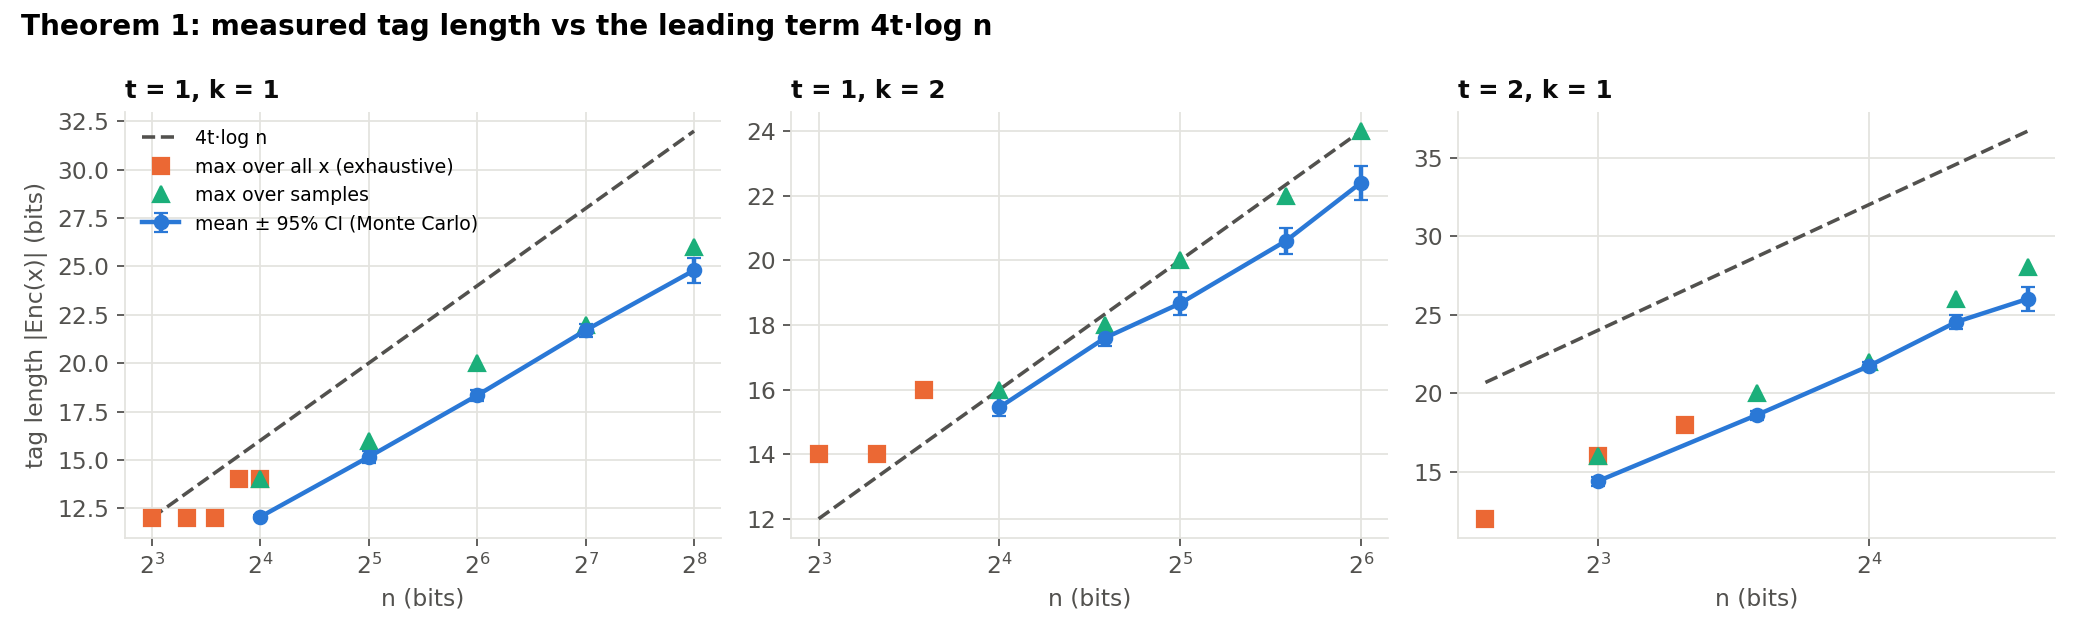
\includegraphics[width=\textwidth]{fig01_thm1_length.png}
\caption{Theorem~\ref{thm:1}: tag length against $n$. Monte Carlo mean $\pm$95\% CI, sampled maximum, exhaustive maximum over all $\bx$, and the leading term $4t\log n$ (dashed).}
\label{fig:thm1len}
\end{figure*}

\begin{table}[!t]
\caption{Theorem~\ref{thm:1}, Monte Carlo (selected rows)}\label{tab:thm1}
\centering\footnotesize
\setlength{\tabcolsep}{3.2pt}
\begin{tabular}{@{}lrrrrrr@{}}
\toprule
$t,k$ & $n$ & mean tag & max & $4t\log n$ & $|\C(\bx)|$ & decoded\\
\midrule
1,1 & 16 & $12.1\pm0.1$ & 14 & 16.0 & 229 & 200/200\\
1,1 & 64 & $18.3\pm0.3$ & 20 & 24.0 & 3{,}905 & 150/150\\
1,1 & 256 & $24.8\pm0.6$ & 26 & 32.0 & 65{,}257 & 50/50\\
1,2 & 16 & $15.4\pm0.3$ & 16 & 16.0 & 803 & 200/200\\
1,2 & 64 & $22.4\pm0.5$ & 24 & 24.0 & 18{,}554 & 50/50\\
2,1 & 8 & $14.4\pm0.3$ & 16 & 24.0 & 221 & 200/200\\
2,1 & 24 & $26.0\pm0.7$ & 28 & 36.7 & 50{,}930 & 40/40\\
\bottomrule
\end{tabular}
\end{table}

\begin{itemize}
\item All 2{,}065 decoding trials succeeded (Table~\ref{tab:thm1}).
\item Tag length (Fig.~\ref{fig:thm1len}): for $k=1$ the exhaustive worst case is $12,12,12,14,14$ bits at $n=8,\dots,16$, against $4t\log n=12,\dots,16$. For $k=2$ the worst string exceeds the leading term at small $n$ ($14,14,16$ against $12,13.3,14.3$ at $n=8,10,12$). Each doubling of $n$ adds $3.2$ bits for $t=1$ (bound: $4$) and $7.5$ bits for $t=2$ (bound: $8$).
\item Confusion ball: fitted slopes $2.04$, $2.25$, $4.97$ for $(t,k)=(1,1),(1,2),(2,1)$, against $2t=2,2,4$.
\item Time: encoding slopes $2.46,2.69,4.58$ (theory $\le3,3,5$); decoding slopes $0.97,1.13,1.89$ (theory $\le2,2,3$).
\end{itemize}

\textbf{Interpretation.} Theorem~\ref{thm:1} holds in the form it is stated. The tag is usually below $4t\log n$ because the modulus found is much smaller than the ball ($a_{\bx}\approx4{,}000$ against $|\C|\approx65{,}000$ at $n=256$). The excess for $k=2$ at small $n$ is allowed by the $o(\log n)$ term: the constant $k^{2t}3^{2kt}=36$ in~\eqref{eq:ballbound} adds about five bits, and the excess is gone by $n=64$.

%---------------------------------------------------------------------
\subsection{Average-Case Scheme (Theorem~\ref{thm:2})}
\textbf{Choices made.}
\begin{enumerate}
\item[(i)] The same labeling function $f(\bx)=\bx$.
\item[(ii)] \emph{Side information $\psi$.} The one-edit code of~\cite{li22} (Lemma~\ref{lem:onecode}) is used as a black box in the theory, so we built a simple stand-in: $\psi(\bx)=(A_{\bx},S_0,S_1)$, where $A_{\bx}$ is the largest part-integer and $S_0,S_1$ are sums of the residues of the even and odd $L$-bit blocks modulo a fixed prime. One-edit recovery then holds with high probability rather than always, but decoding of the full scheme stays correct, since $\psi$ is used only to filter candidates. We use $L=8192$ ($k=1$) and $L=16384$ ($k=2$).
\item[(iii)] \emph{Restricted ball.} $\Ct(\bx)$ keeps the strings of $\C(\bx)$ that are dense and have the same $h$ and the same $\psi$, as Lemma~\ref{lem:restricted} requires.
\item[(iv)] \emph{Density threshold.} The paper's $\delta=k2^{2k+3}\log n$ exceeds $n$ for $n<256$ ($k=1$), so every string we can encode is dense; the unit tests use a small $\delta$ to also exercise the non-dense branch.
\end{enumerate}

\textbf{Important code} (\path{schemes/average_case/scheme.py}):
\par\noindent\begin{minipage}{\columnwidth}\scriptsize
\begin{verbatim}
def encode(x):
    if not is_dense(x, k, delta):       # rare
        return (0,) + worst_case_tag(x)
    C = [z for z in confusion_ball(x, k, t)
         if is_dense(z) and h(z) == h(x)
         and psi(z) == psi(x)]          # restricted ball
    a = find_modulus(f(x), [f(z) for z in C if z != x])
    return (1, h(x), psi(x), f(x) % a, a)
\end{verbatim}
\end{minipage}\par
\noindent\begin{minipage}{\columnwidth}\scriptsize
\begin{verbatim}
def decode(y, (1, hx, px, r, a), n):
    S = [z for z in suspects(y, n, k, t)
         if is_dense(z) and h(z) == hx and psi(z) == px]
    return the unique z in S with f(z) % a == r
\end{verbatim}
\end{minipage}\par

\textbf{Inputs and outputs.} As for the worst case, plus $\delta$ and $L$. Output: the tag $(\text{flag},h,\psi,r,a)$ with the length of each part, and $|\Ct(\bx)|$.

\textbf{Verification strategy.} A bound of the form ``leading term $+\,o(\log n)$'' cannot be checked at a single $n$. We therefore check (a) that the slope of the average tag length against $\log n$ is at most $4t-1$; (b) that the remainder (length $-$ leading term)$/\log n$ decreases with $n$; and (c) each ingredient against its own lemma: density (Lemma~\ref{lem:dense}), one-edit recovery (Lemma~\ref{lem:onecode}) and the size of $\Ct(\bx)$ (Lemma~\ref{lem:restricted}). Script: \path{experiments/verify_average_case.py}.

\textbf{Results.}
\begin{figure*}[!t]
\centering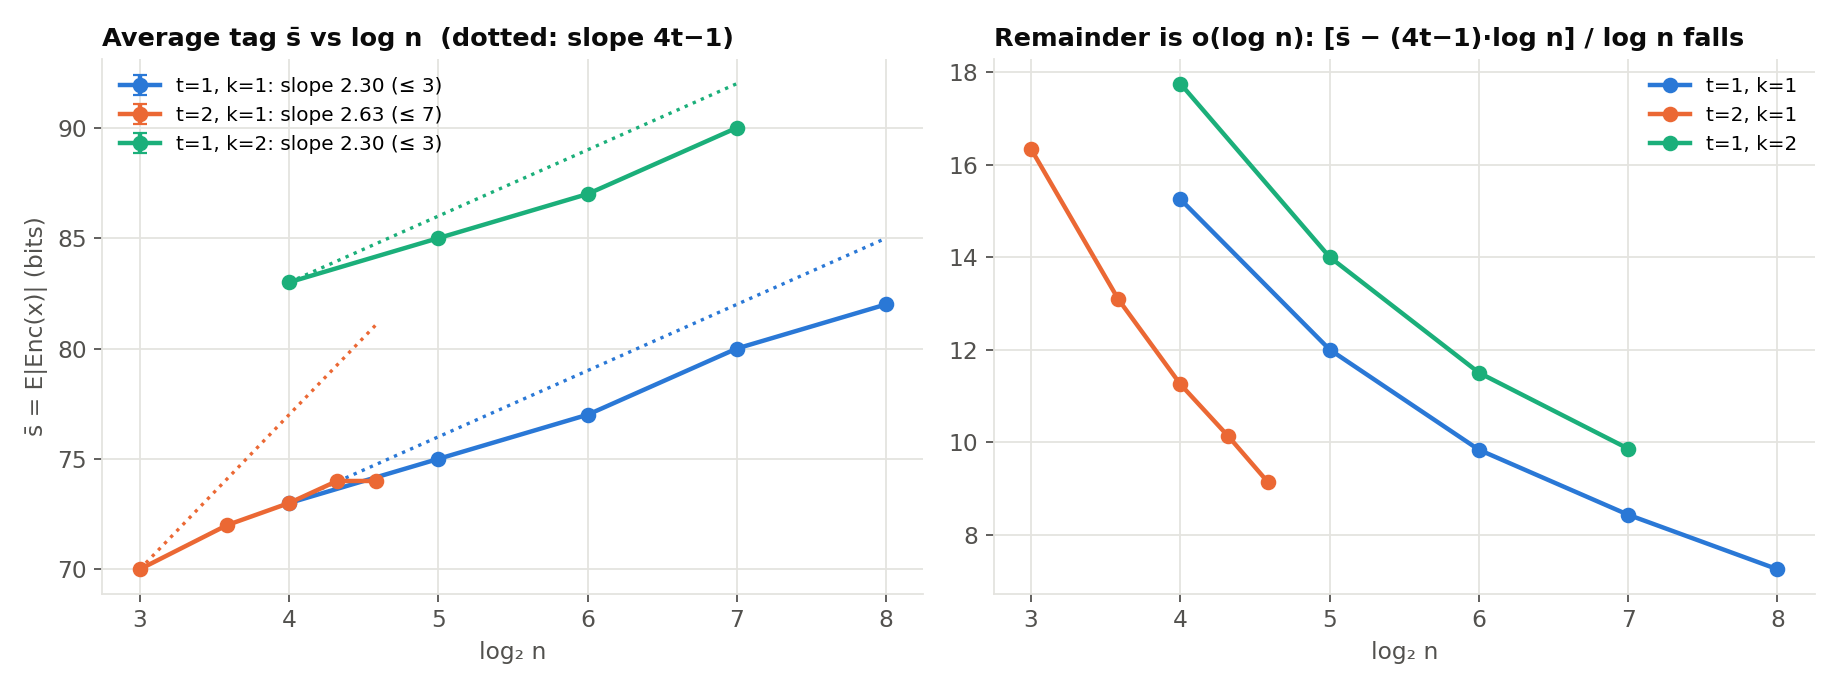
\includegraphics[width=0.92\textwidth]{fig06_thm2_length.png}
\caption{Theorem~\ref{thm:2}: average tag length $\bar s$ against $\log n$ with fitted slopes (dotted: slope $4t-1$), and the remainder $[\bar s-(4t-1)\log n]/\log n$.}
\label{fig:thm2}
\end{figure*}

\begin{table}[!t]
\caption{Theorem~\ref{thm:2}: verification checks}\label{tab:checks}
\centering\footnotesize
\setlength{\tabcolsep}{3pt}
\begin{tabular}{@{}lccc@{}}
\toprule
Check & $t{=}1,k{=}1$ & $t{=}2,k{=}1$ & $t{=}1,k{=}2$\\
\midrule
C1 every tag decodes & pass & pass & pass\\
C2 $(r,a)\le(4t-2)\log n$ & pass (3 b) & pass & pass\\
C3 $|h|-\log n$ constant & pass (31) & pass & pass (36)\\
C4 slope $\le 4t-1$ & $2.30\le3$ & $2.63\le7$ & $2.30\le3$\\
C5 remainder$/\log n$ falls & $15.2\to7.2$ & $16.3\to9.1$ & $17.8\to9.9$\\
\bottomrule
\end{tabular}
\end{table}

\begin{itemize}
\item \emph{Density}: the non-dense fraction falls from 72\% at $\delta=10$ to 0.05\% at $\delta=24$ ($k=1$, $n=256$). At the paper's $\delta$ the union bound is $7\cdot10^{-18}$ for $n=1024$, far below the claimed $O(n^{-3})$.
\item \emph{One-edit recovery}: for $k=1$, $\bx$ was recovered in 60/60, 60/60, 50/60 and 23/25 trials at $n=2^{12},2^{14},2^{16},2^{18}$, with no wrong output; every failure was a localisation window spanning more than two $\psi$-blocks.
\item \emph{Theorem~\ref{thm:2}} (Fig.~\ref{fig:thm2}, Table~\ref{tab:checks}): all 1{,}630 decodes succeeded; the slopes are within $4t-1$ and the remainder falls relative to $\log n$.
\item \emph{Restricted ball}: ``dense and same $h$'' leaves 1--12 of 225--64{,}083 confusable strings ($n=16$--$256$), below $n^{2t-1}$; adding ``same $\psi$'' leaves only $\bx$, so $(r,a)$ costs 3 bits.
\item \emph{Bit budget}: at $n=256$ the tag is $1+39\,(h)+39\,(\psi)+3=82$ bits, against 25 bits for Theorem~\ref{thm:1}. From the measured part sizes, the average-case scheme becomes shorter only near $n\approx2^{108}$.
\end{itemize}

\textbf{Interpretation.} Theorem~\ref{thm:2} holds as stated: the leading term is $(4t-1)\log n$ and the rest grows more slowly than $\log n$. The saving of one $\log n$ is, however, paid for by about 70 bits of side information ($h$ and $\psi$), so at every size we can run it is longer than the worst-case scheme. Lemma~\ref{lem:dense} is correct but loose by many orders of magnitude.

%---------------------------------------------------------------------
\subsection{Higher-Complexity Scheme of~\cite{li21}}\label{sec:li21}
\textbf{Methodology.} A valid scheme is a proper colouring of the confusion graph, and the tag is the colour of $\bx$ (Proposition~\ref{prop:colour}). Scheme~\cite{li21} computes the colour of one string with two rounds of Linial-type recolouring. Each colour $i$ is mapped to a polynomial $g_i$ over $\mathbb F_Q$ whose coefficients are the base-$Q$ digits of $i$, and the new colour of $\bx$ is $(\alpha,g_{c(\bx)}(\alpha))$ for the smallest $\alpha$ at which $g_{c(\bx)}$ differs from the polynomials of all neighbours' colours (the \emph{witness}). Round~1 starts from the string itself ($Q_1>\Delta n$); round~2 starts from the round-1 colour ($Q_2>\Delta\lceil\log Q_1^2\rceil$). The tag is the round-2 colour, $\lceil\log Q_2^2\rceil$ bits. Bob lists his suspects and keeps the one with the received colour.

\textbf{Choices made.} (i) $\Delta$ is the \emph{exact} maximum degree of the confusion graph, computed once per $(n,k,t)$ by enumerating all $2^n$ strings; the paper's asymptotic bound would be about 40 times larger here and cost about 10 more bits. (ii) $Q$ is the smallest prime above $\Delta b$. (iii) Two rounds, as in the paper. (iv) Block lengths up to $16$ bits, since $\Delta$ requires all $2^n$ strings.

\textbf{Important code} (\path{schemes/li21.py}):
\par\noindent\begin{minipage}{\columnwidth}\scriptsize
\begin{verbatim}
def colour(x):                     # the tag of x
    c1 = lambda z: witness(int(z), neighbours(z), Q1)
    return witness(c1(x), [c1(z) for z in neighbours(x)],
                   Q2)
\end{verbatim}
\end{minipage}\par
Here \texttt{neighbours}$(\bz)=\C(\bz)\setminus\{\bz\}$; round-1 colours are cached, since one colour needs the round-1 colours of all neighbours.

\textbf{Inputs and outputs.} Blocks of $n=8$--$16$ bits with $t=k=1$. Output: the colour and its length.

\textbf{Verification.} The tests check the witness property, that the colouring is proper on all $256$ strings of length $8$ (every confusable pair gets different colours), and random round trips.

\textbf{Results.} At $n=8$: $\Delta=64$, $Q_1=521$, $Q_2=1217$, a $21$-bit tag. At $n=16$: $\Delta=292$ and a $26$-bit tag; computing $\Delta$ takes $36$\,s once, and a block takes about $0.15$\,s to encode and $1$\,s to decode.

\textbf{Interpretation.} The scheme is optimal only asymptotically: its $O(\log\log n)$ term hides the factor $b$ in $Q>\Delta b$, which costs about $2\log n$ bits at these sizes.

%---------------------------------------------------------------------
\subsection{Comparison on Synthetic Edited Data}\label{sec:compare}
\textbf{Set-up.} \path{experiments/compare.py} runs the three schemes on the \emph{same} random blocks with the \emph{same} random edits: $t=k=1$, $n=8,10,\dots,16$, $15$ strings per length and $3$ edit patterns per string. The block length is limited by scheme~\cite{li21}.

\begin{table}[!t]
\caption{Three schemes on the same synthetic blocks ($t=k=1$)}\label{tab:compare}
\centering\footnotesize
\setlength{\tabcolsep}{3pt}
\begin{tabular}{@{}rrrrrrr@{}}
\toprule
 & \multicolumn{3}{c}{tag length (bits)} & & \multicolumn{2}{c}{\cite{li21}: time per block}\\
\cmidrule(lr){2-4}\cmidrule(l){6-7}
$n$ & Thm~\ref{thm:1} & Thm~\ref{thm:2} & \cite{li21} & $4t\log n$ & encode & decode\\
\midrule
8 & 10.0 & 70 & 21 & 12.0 & 0.9\,ms & 1.0\,ms\\
10 & 10.1 & 72 & 23 & 13.3 & 4.5\,ms & 6.3\,ms\\
12 & 11.2 & 72 & 24 & 14.3 & 17\,ms & 30\,ms\\
14 & 12.1 & 73 & 25 & 15.2 & 47\,ms & 128\,ms\\
16 & 12.4 & 73 & 26 & 16.0 & 121\,ms & 444\,ms\\
\bottomrule
\end{tabular}
\end{table}

\begin{figure}[!t]
\centering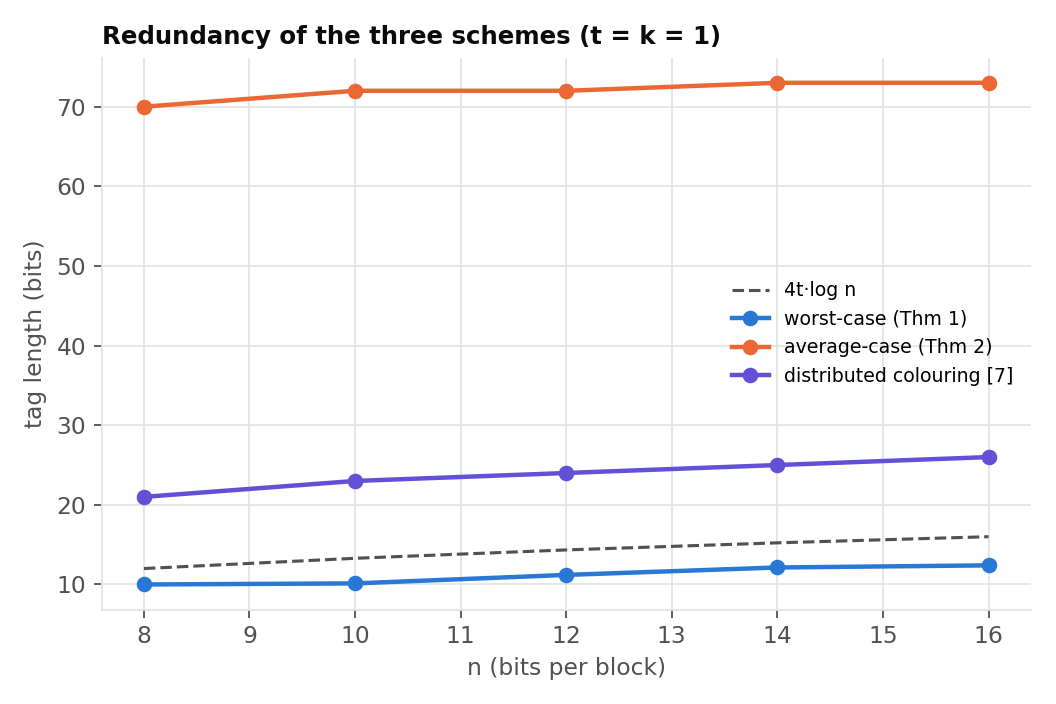
\includegraphics[width=\columnwidth]{fig10_compare_redundancy.png}
\caption{Tag length of the three schemes on the same blocks ($t=k=1$), with the leading term $4t\log n$.}
\label{fig:compare}
\end{figure}

\begin{figure}[!t]
\centering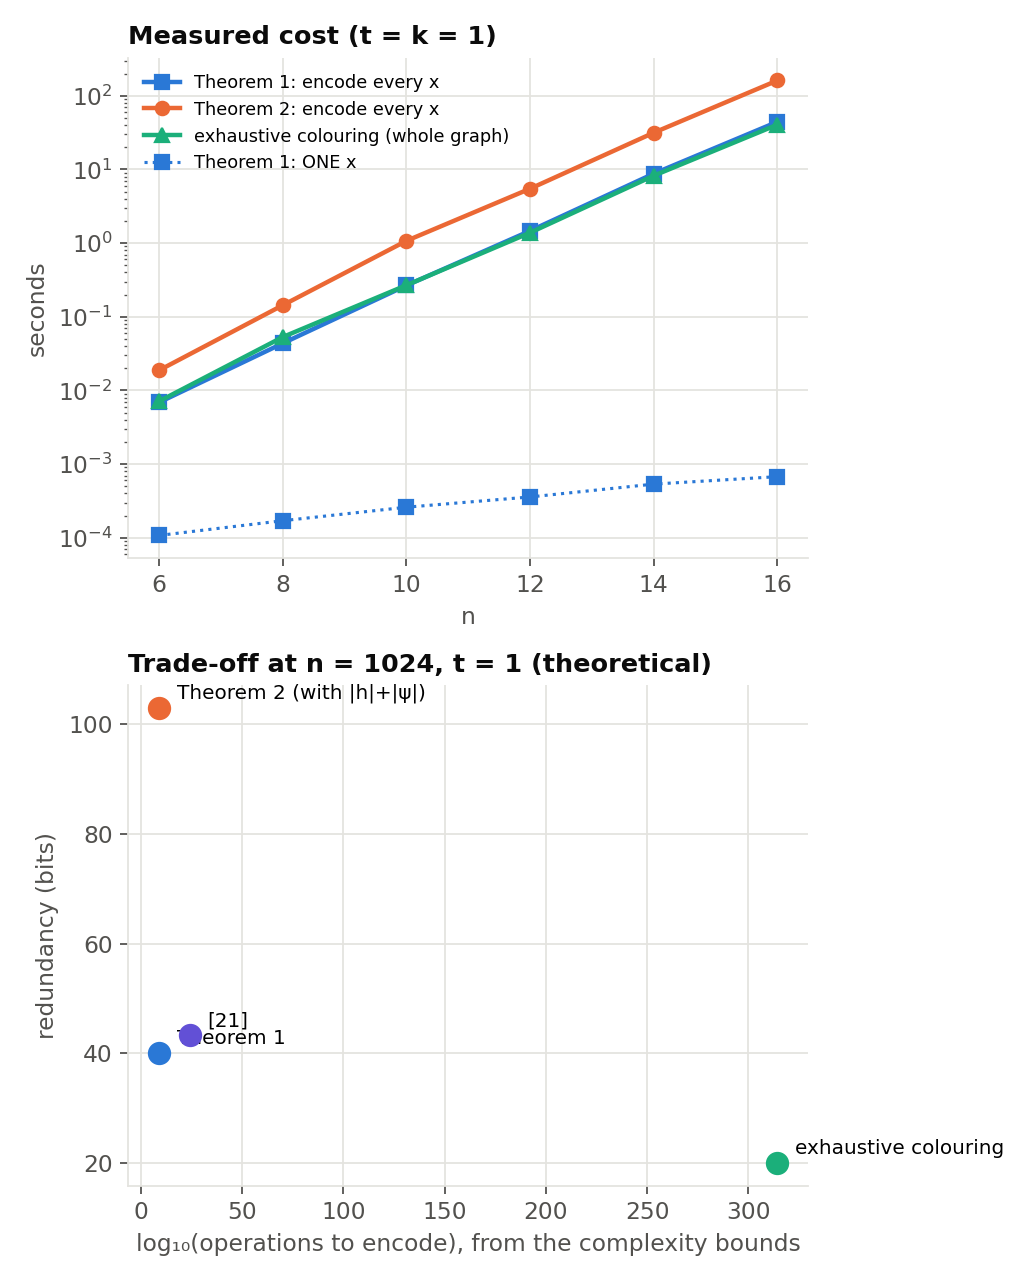
\includegraphics[width=\columnwidth]{fig11_compare_cost.png}
\caption{Encoding and decoding time per block (log--log) with fitted slopes.}
\label{fig:cost}
\end{figure}

\textbf{Results.} All $675$ decodings succeeded (Table~\ref{tab:compare}, Figs.~\ref{fig:compare},~\ref{fig:cost}).
\begin{itemize}
\item \emph{Redundancy:} Theorem~\ref{thm:1} ($10$--$12$ bits) $<$ scheme~\cite{li21} ($21$--$26$ bits) $<$ Theorem~\ref{thm:2} ($70$--$73$ bits) at every $n$.
\item \emph{Complexity:} fitted slopes of encoding time are $2.0$, $2.4$ and $7.1$, and of decoding time $1.2$, $1.1$ and $8.8$ (Theorem~\ref{thm:1}, Theorem~\ref{thm:2}, \cite{li21}). At $n=16$, scheme~\cite{li21} is about $200$ times slower to encode and $20{,}000$ times slower to decode than Theorem~\ref{thm:1}.
\end{itemize}

\textbf{Interpretation.} All three schemes have the leading term $4t\log n$ or less, so the differences come from the lower-order terms. Theorem~\ref{thm:1} needs only one confusion ball and its modulus is far smaller than the ball, so it is both the shortest and the fastest. Scheme~\cite{li21} pays about $2\log b$ bits for $Q>\Delta b$, and its cost is high because the colour of $\bx$ needs the round-1 colours of all $\Delta$ neighbours, i.e.\ about $\Delta^2=O(n^{4t})$ ball enumerations. Theorem~\ref{thm:2} pays a fixed $\approx70$ bits for $h$ and $\psi$. Asymptotically, scheme~\cite{li21} has the smaller remainder and Theorem~\ref{thm:2} the smaller leading term, but at the sizes where all three can be run, the worst-case scheme is best on both counts.

\subsubsection{Two hand-edited documents}\label{sec:docs}
To check the schemes on edits made by hand rather than by the random channel, we made two documents.

\textbf{Choices made.} (i) \emph{Binary documents}: each document is a text file of the characters \texttt{0} and \texttt{1}; in ordinary text one character is $8$ bits, which would need $k\ge8$ and a confusion ball too large to enumerate. (ii) \emph{One block per line}: each line is a $16$-bit block encoded separately, so an insertion or deletion stays inside its line and does not shift the other blocks. (iii) \emph{Same blocks for all three schemes}, with $t=k=1$.

\textbf{Inputs and outputs.} Each document (\path{documents/doc1}, \path{documents/doc2}) has an \path{original.txt} of $8$ random $16$-bit lines and an \path{edited.txt} changed by hand with at most one bit inserted, deleted or flipped per line. \path{doc1} received 3 insertions, 2 deletions and 2 flips; \path{doc2} 3 insertions, 3 deletions and 1 flip; one line of each was left unchanged. The script \path{experiments/run_documents.py} outputs, per block and scheme, the tag length, whether the line was recovered, and the times.

\begin{table}[!t]
\caption{The three schemes on the two hand-edited documents ($8$ blocks of $16$ bits, $t=k=1$)}\label{tab:docs}
\centering\footnotesize
\setlength{\tabcolsep}{3pt}
\begin{tabular}{@{}llrrrr@{}}
\toprule
Doc. & Scheme & total tag & recovered & encode & decode\\
\midrule
doc1 & Thm~\ref{thm:1} & 98 bits & 8/8 & $<0.01$\,s & $<0.01$\,s\\
 & Thm~\ref{thm:2} & 584 bits & 8/8 & 0.06\,s & $<0.01$\,s\\
 & \cite{li21} & 208 bits & 8/8 & 1.1\,s & 6.5\,s\\
\midrule
doc2 & Thm~\ref{thm:1} & 96 bits & 8/8 & 0.01\,s & $<0.01$\,s\\
 & Thm~\ref{thm:2} & 584 bits & 8/8 & 0.02\,s & $<0.01$\,s\\
 & \cite{li21} & 208 bits & 8/8 & 1.4\,s & 6.9\,s\\
\bottomrule
\end{tabular}
\end{table}

\begin{figure}[!t]
\centering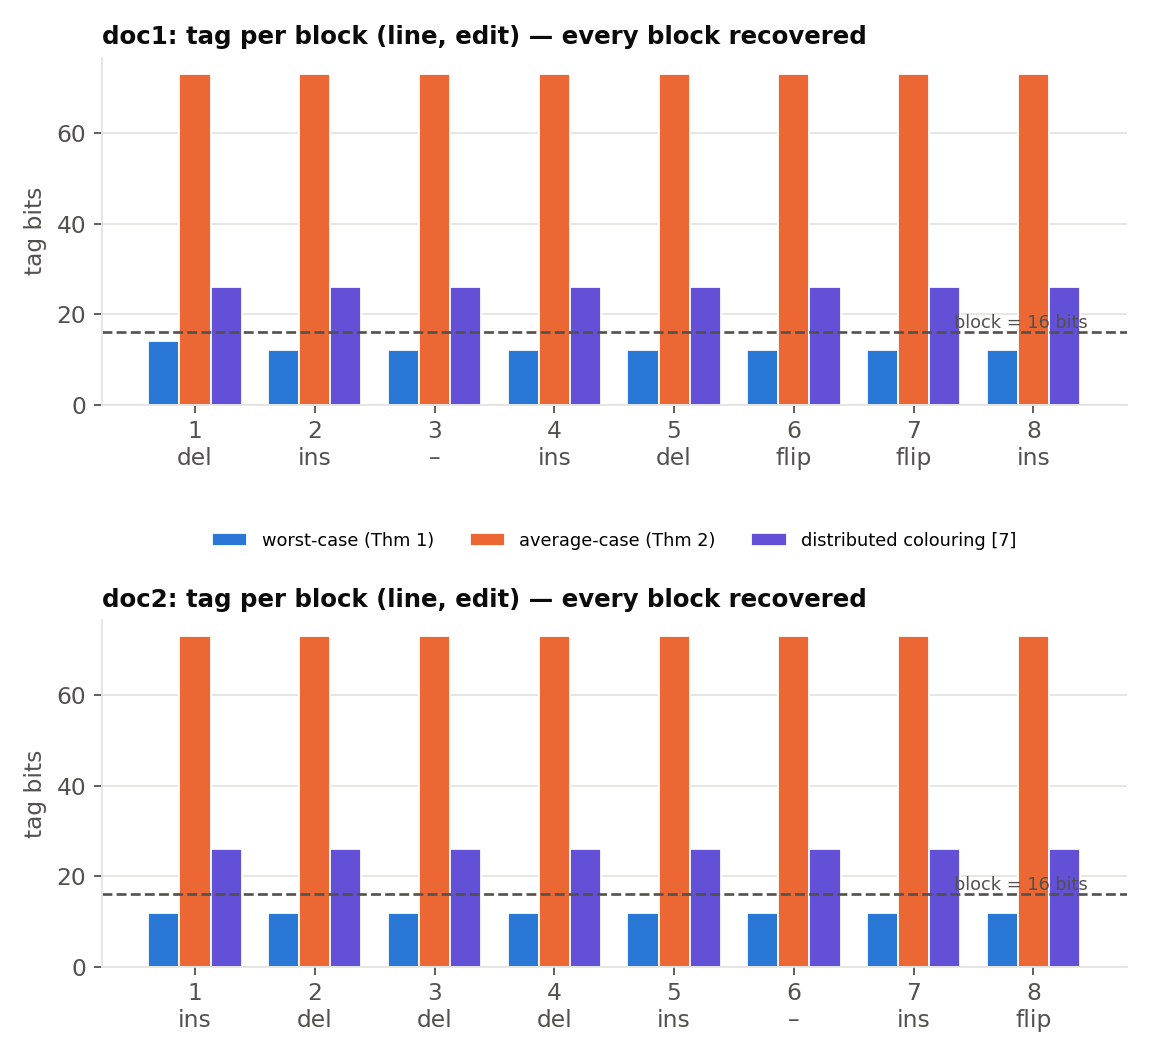
\includegraphics[width=\columnwidth]{fig15_documents.png}
\caption{Tag length per block for each document, labelled with the line number and the edit made (\emph{ins}, \emph{del}, \emph{flip}, or none); the dashed line is the block length.}
\label{fig:docs}
\end{figure}

\textbf{Results.} Every scheme recovered all $16$ blocks, for insertions, deletions and flips alike (Table~\ref{tab:docs}, Fig.~\ref{fig:docs}). The total tag for a $128$-bit document is $96$--$98$ bits for Theorem~\ref{thm:1}, $208$ for~\cite{li21} and $584$ for Theorem~\ref{thm:2}, the same per-block lengths as in Table~\ref{tab:compare} at $n=16$.

\textbf{Interpretation.} The tags are large relative to the documents because the blocks are short ($4\log16=16$ bits equals the block length) and every block needs its own tag, since Alice does not know which lines changed. Splitting is still worthwhile here: with seven edits per document, a single Theorem~\ref{thm:1} tag for the whole document would need about $4\cdot7\cdot\log128=196$ bits.

%---------------------------------------------------------------------
\subsection{Conclusion of the Implementation}
Both schemes of~\cite{narayanan} were implemented and decoded every test case, and their encoding lengths follow Theorems~\ref{thm:1} and~\ref{thm:2}: the worst-case tag stays near or below $4t\log n$, and the average-case tag has leading term $(4t-1)\log n$. Against the higher-complexity scheme of~\cite{li21} on the same synthetic and hand-edited data, the worst-case scheme has the shortest tag and the lowest running time; the average-case scheme is the longest because of its fixed side information, and scheme~\cite{li21} is the slowest by several orders of magnitude.

%=====================================================================
\section{Extension: Real Version-Control Data}\label{sec:ext}
\textbf{Question.} Do the edits people actually make fit the model of~\cite{narayanan}, a few ($t$) substring edits of at most $k$ bits each, or do real edit patterns break its assumptions?

{\sloppy\textbf{Data and method.} We used the full history (all branches) of one of our own local git repositories, a course project written in Verilog, Python, Makefiles and Markdown. For every non-merge commit and every modified text file we took the file before (parent) and after (commit): 101 file changes in 31 commits, median file 6.6\,KB ($n\approx53{,}000$ bits). Only statistics are recorded (\path{results/ext_*.csv}); no file contents or names. For each change (\path{io/diffs.py}): a line-level then byte-level diff gives the changed regions in bits; $t_{\min}(k)$, the fewest $k$-substring edits turning the old file into the new, is found by dynamic programming over groups of neighbouring regions (a group spanning $s$ bits needs $\lceil s/k\rceil$ edits). A change \emph{fits} $(t,k)$ if $t_{\min}(k)\le t$; one that does not is a model violation, not a decoder failure. We also check the line view of Sec.~\ref{sec:docs}, the density precondition of Theorem~\ref{thm:2}, and run the three schemes on real single-bit edits (\path{experiments/extension_commits.py}).\par}

\begin{table}[!t]
\caption{Share of real file changes that fit $t$ edits of $\le k$ bits}\label{tab:fit}
\centering\footnotesize
\begin{tabular}{@{}lrrrr@{}}
\toprule
$k$ (bits) & $t\le1$ & $t\le2$ & $t\le3$ & $t\le5$\\
\midrule
1, 2, 4 & 0\% & 0\% & 0\% & 0\%\\
8 & 0\% & 0\% & 0\% & 1\%\\
64 & 1\% & 3\% & 4\% & 5\%\\
512 & 5\% & 9\% & 16\% & 33\%\\
4096 & 26\% & 48\% & 62\% & 75\%\\
\bottomrule
\end{tabular}
\end{table}

\begin{figure}[!t]
\centering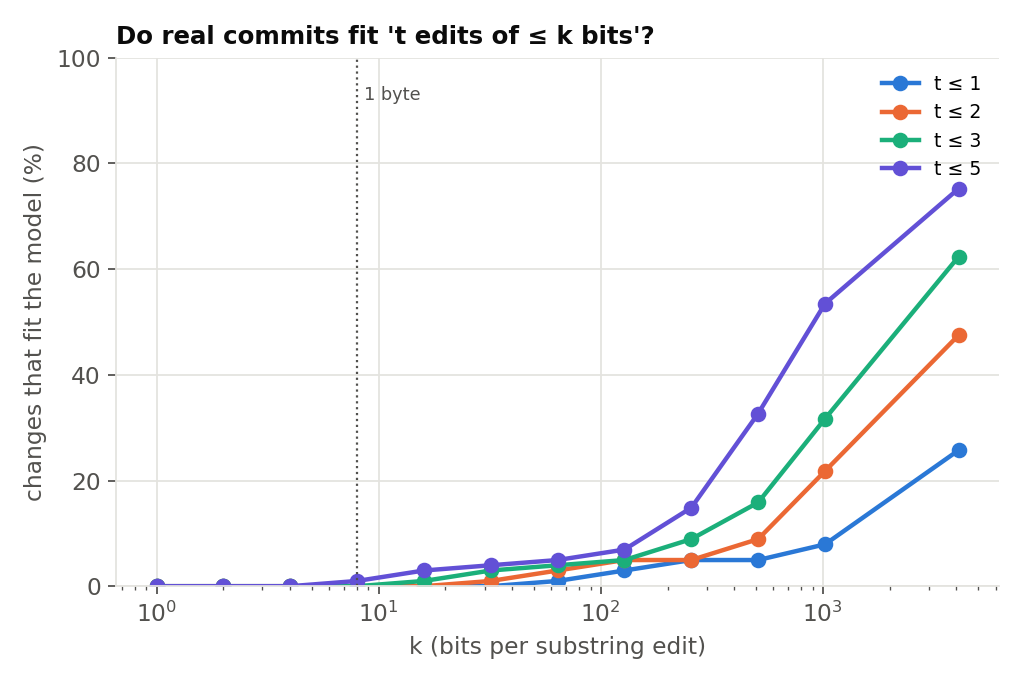
\includegraphics[width=\columnwidth]{fig12_real_fit.png}
\caption{Share of real file changes that fit the $(t,k)$ model, against $k$.}
\label{fig:fit}
\end{figure}

\textbf{Findings} (Table~\ref{tab:fit}, Fig.~\ref{fig:fit}).

(1) \emph{Edits are few but long.} A median change touches 4 regions but 3{,}231 bits, and its largest region is 1{,}768 bits. No change fits $k\le4$ for any $t\le5$, and at most 3\% fit $k\le32$; a median change needs $t_{\min}=398$ edits at $k=8$ and $52$ at $k=64$. Even with $k=512$ bits only 16\% fit $t\le3$. The small constant $k$ of the paper is the assumption real data breaks.

(2) \emph{Lines are added, not just edited.} 100 of the 101 changes add or remove whole lines (97 add), so the one-block-per-line layout of Sec.~\ref{sec:docs}, which needs the number of lines to stay fixed, also breaks. Of the 375 lines that are changed in place, 43 (11\%) are one edit of $\le8$ bits and 103 (27\%) one edit of $\le64$ bits.

(3) \emph{At the $k$ real edits need, the constant dominates.} For changes fitting $t\le3$, the estimated tag has median 966 bits at $k=64$ (against $4t\log n\approx84$) and 6{,}738 bits at $k=512$ (against 139), because of the $3^{2kt}$ factor in~\eqref{eq:ballbound}. On small files it exceeds the file itself.

(4) \emph{Density holds.} All 101 old files are dense for $k=1$ and $k=2$ at the paper's $\delta$: the longest gap between $0^k1^k$ patterns is at most 11 bits for $k=1$ (median 10), against $\delta\approx500$. Real text, though far from uniform, meets the precondition of Theorem~\ref{thm:2}.

(5) \emph{Where an edit is small, the schemes work.} We cut 16-bit windows of the old file around 40 isolated real single-bit edits (all flips) and ran the three schemes with $t=k=1$. All 40 were recovered by every scheme, with tags of 11.9 (Thm.~1), 73.0 (Thm.~2) and 26.0 bits~\cite{li21}, as on synthetic data (Sec.~\ref{sec:compare}).

\textbf{Answer.} The \emph{form} of the model, a few localised substring edits, matches real commits; its \emph{scale} does not. Real edits insert whole lines of hundreds to thousands of bits, so $k$ must be large and the $3^{2kt}$ term outweighs $4t\log n$. Density holds; bounded $k$ breaks.

%=====================================================================
\FloatBarrier
\section{Limitations and Observations on the Reference}\label{sec:limits}
\textbf{Limitations.} The labeling function and the block hash in $\psi$ are stand-ins (Sec.~\ref{sec:impl}); scheme~\cite{li21} uses the exact maximum degree, which requires enumerating all $2^n$ strings and limits it to blocks of about $16$ bits; brute-force enumeration limits the low-complexity schemes to $n\le256$ ($t=1$) and $n\le24$ ($t=2$); on documents, every block needs its own tag, so the total redundancy grows linearly with the document length; the paper's $\delta$ exceeds $n$ at encodable sizes; the real data is one repository (101 file changes), the real-data tag is an estimate, and the real windows are selected small edits. Multi-round protocols and non-uniform source models were not attempted.

\textbf{Observations on~\cite{narayanan}.} (i) The ``no extra cost'' search for $a_{\bx}$ needs re-checking of earlier neighbours. (ii) Theorem~2 refers to ``$a_{\bx}$ as in Lemma~2''; Lemma~1 is meant. (iii) The average redundancy should be normalised by $2^n$, not $n$. (iv) The restricted confusion ball needs ``same $h,\psi$'' for Lemma~\ref{lem:restricted}. (v) Lemma~\ref{lem:dense}'s bound is valid but loose by many orders of magnitude.

%=====================================================================
\section{Conclusion}
Both schemes of~\cite{narayanan} work as claimed: every tag decoded, the confusion ball grows as $n^{2t}$, the complexities hold, and both redundancy bounds are verified in the form they are stated. The experiments also show what the asymptotic statements hide. $4t\log n$ is a leading term that small-$n$, $k=2$ cases exceed; the average-case scheme saves $\log n$ only after paying about 70 bits of side information, so it overtakes the worst-case scheme near $n\approx2^{108}$; and the low-complexity scheme pays 2--2.5 times the redundancy of an exhaustive colouring in return for polynomial running time. On real version-control history the substring-edit model fits in form but not in scale: real edits add whole lines and need $k$ in the hundreds of bits.

%=====================================================================
\appendix[Reproducing the Results]
{\raggedright
\begin{itemize}
\item \texttt{python3 run\_all.py}: unit tests and all experiments (about 15\,min; add \texttt{--quick} for a one-minute check).
\item \texttt{python3 experiments/extension\_commits.py --repo PATH}: the extension on any local git repository (only statistics are written).
\item \texttt{python3 experiments/figures.py}: draws every figure (needs matplotlib).
\end{itemize}
Seeds are fixed, so reruns reproduce the reported numbers.\par}

\begin{table}[!t]
\caption{Build sequence of the implementation (one commit per row)}\label{tab:build}
\centering\footnotesize
\begin{tabular}{@{}r>{\raggedright\arraybackslash}p{0.47\columnwidth}>{\raggedright\arraybackslash}p{0.33\columnwidth}@{}}
\toprule
\# & Component & Checked by\\
\midrule
1 & Project skeleton & --\\
2 & Edit model: $\B_t$, $\C_t$ via~\eqref{eq:identity}, Bob's suspects, channel (\path{core/edits.py}) & Example~1; Eq.~\eqref{eq:identity} vs.\ Def.~2 for all $n\le6$\\
3 & Labeling $f(\bx)=\bx$ and syndrome compression (\path{core/labeling.py}, \path{core/syndrome.py}) & Toy example $a=7$; smallest valid $a$; $a\le2MR\ln(MR)$\\
4 & Common scheme interface; worst-case scheme (\path{schemes/base.py}, \path{schemes/worst_case.py}) & Example $\bx=10110\to(9,13)$; all $\bx\in\{0,1\}^8$, all $\by\in\B_1(\bx)$\\
5 & Verification of Theorem~\ref{thm:1}: Monte Carlo and exhaustive runs, figures (\path{experiments/verify_worst_case.py}) & 2{,}065/2{,}065 decoded; Fig.~\ref{fig:thm1len}\\
6 & Density: partition at $0^k1^k$, both density forms, Lemma~\ref{lem:dense} bound (\path{schemes/average_case/density.py}) & Example of~\cite{li22}; brute force; bound $<n^{-3}$\\
7 & Hash $h$ and localisation (\path{schemes/average_case/hash_h.py}) & Edit always inside the located window\\
8 & Side information $\psi$ and the one-edit decoder (\path{schemes/average_case/psi.py}) & One edit recovered at $n=2^{13}$; never a wrong output\\
9 & Average-case scheme: restricted ball, encoder, decoder (\path{schemes/average_case/scheme.py}) & Both branches decode; survivors $\subseteq\Ct(\bx)$\\
10 & Verification of Theorem~\ref{thm:2} and Lemmas~\ref{lem:dense}--\ref{lem:restricted}, figures (\path{experiments/verify_average_case.py}) & Checks C1--C5 pass (Table~\ref{tab:checks})\\
11 & Higher-complexity scheme of~\cite{li21}: two-round distributed colouring (\path{schemes/li21.py}) & Proper colouring on all $2^8$ strings; round trips\\
12 & Binary documents, one block per line, edit-model check (\path{io/documents.py}, \path{documents/}) & Hand-worked edit counts; block classification\\
13 & Comparison of the three schemes on synthetic blocks, figures (\path{experiments/compare.py}) & 675/675 decoded; slopes in Fig.~\ref{fig:cost}\\
14 & The three schemes on the two hand-edited documents, figure (\path{experiments/run_documents.py}) & All $16$ blocks recovered by every scheme\\
15 & Extension on real version-control history: diffs to $k$-substring edits, $t_{\min}(k)$, density, real windows (\path{io/diffs.py}, \path{core/bounds.py}, \path{experiments/extension_commits.py}) & Hand-worked diffs; Lemma~\ref{lem:ball} bound value; 40/40 real windows decoded\\
\bottomrule
\end{tabular}
\end{table}

\begin{thebibliography}{9}
\bibitem{narayanan} H.~Narayanan, V.~Ramkumar, R.~Bitar, and A.~Wachter-Zeh, ``Coding schemes for document exchange under multiple substring edits,'' arXiv:2601.18441, 2026.
\bibitem{orlitsky} A.~Orlitsky, ``Interactive communication: Balanced distributions, correlated files, and average-case complexity,'' in \emph{Proc. IEEE FOCS}, 1991, pp.~228--238.
\bibitem{cormode} G.~Cormode, M.~Paterson, S.~C.~Sahinalp, and U.~Vishkin, ``Communication complexity of document exchange,'' in \emph{Proc. ACM-SIAM SODA}, 2000, pp.~197--206.
\bibitem{sima_del} J.~Sima, R.~Gabrys, and J.~Bruck, ``Optimal systematic $t$-deletion correcting codes,'' in \emph{Proc. IEEE ISIT}, 2020, pp.~769--774.
\bibitem{sima_sc} J.~Sima, R.~Gabrys, and J.~Bruck, ``Syndrome compression for optimal redundancy codes,'' in \emph{Proc. IEEE ISIT}, 2020, pp.~751--756.
\bibitem{tang} Y.~Tang, S.~Motamen, H.~Lou, K.~Whritenour, S.~Wang, R.~Gabrys, and F.~Farnoud, ``Correcting a substring edit error of bounded length,'' \emph{IEEE Trans. Commun.}, vol.~73, no.~1, pp.~12--21, 2025.
\bibitem{li21} Y.~Li, R.~Gabrys, and F.~Farnoud, ``Constructing low-redundancy codes via distributed graph coloring,'' arXiv:2512.04197, 2025.
\bibitem{li22} Y.~Li, Y.~Tang, H.~Lou, R.~Gabrys, and F.~Farnoud, ``Optimal codes correcting a substring edit,'' \emph{IEEE Trans. Inf. Theory}, vol.~71, no.~7, pp.~5178--5191, 2025.
\end{thebibliography}

\end{document}
